\documentclass[12pt]{article}

\usepackage{fontawesome}
\usepackage{hyperref}
\usepackage{xurl}
\usepackage{graphicx}
\usepackage{float}
\usepackage[tagged, highstructure]{accessibility}
\usepackage{bookmark}
\usepackage{enumitem}

\hypersetup{
    colorlinks=false,
    pdfborder={0 0 0},
    pdftitle={Physical and Device Security},
    pdfauthor={Adrianna Holden-Gouveia},
    pdfsubject={Information Security - Lab Assignment},
    pdflang={en-US},
    pdfkeywords={physical security, IoT, secure boot, signed apps, updates, device disposal}
}

% Configure PDF bookmarks for navigation
\bookmarksetup{
    numbered,
    open,
}

% Configure list spacing for better accessibility
\setlist{nosep}



\title{Physical and Device Security}
\author{
        Adrianna Holden-Gouveia \\
        Website: \href{https://aholdengouveia.name}{aholdengouveia.name}\\ 
        \date{\vspace{-5ex}}
        %Email: \href{mailto:admin@aholdengouveia.name}{admin@aholdengouveia.name} \\
%        \faLinkedin{: aholdengouveia} \\
        \faGithub {: aholdengouveia} \\
        \faTwitter {: aholdengouveia} \\
        }

%S\date{\today}


\begin{document}    

\maketitle

\section*{Accessibility Notice}
This document is also available in HTML format at:

Link: \href{https://aholdengouveia.name/InfoSec/labs/physicalsecurity.html}{\textbf{\nolinkurl{https://aholdengouveia.name/InfoSec/labs/physicalsecurity.html}}}

The HTML version provides enhanced accessibility features including keyboard navigation, screen reader support, responsive design, dark mode support, and high contrast options.

\section*{Learning Outcomes}
By the end of this lab, you will be able to:
\begin{itemize}
    \item Identify the connected devices in a home, and the risks each one brings
    \item Check and improve the update and startup protections on your own computer and phone
    \item Explain how secure boot, signed apps, and automatic updates protect a device
    \item Plan how to safely wipe and get rid of old devices, including printers and copiers
\end{itemize}

\section*{Lab Instructions}
If someone can touch a device, they can usually get into it. In this lab, you'll look at the devices around you: the connected devices in your home, the protections on your own computer and phone, and what happens to devices when you're done with them.

\subsection*{Screenshots}
This lab asks for about 10 screenshots. Each screenshot should have your name, term, and year.  One of the easiest ways to do that is make a text document with your name and term/year on your computer and save it to use all term. Any screenshots that don't include this information won't be counted.

\begin{figure}[H]
    \centerline{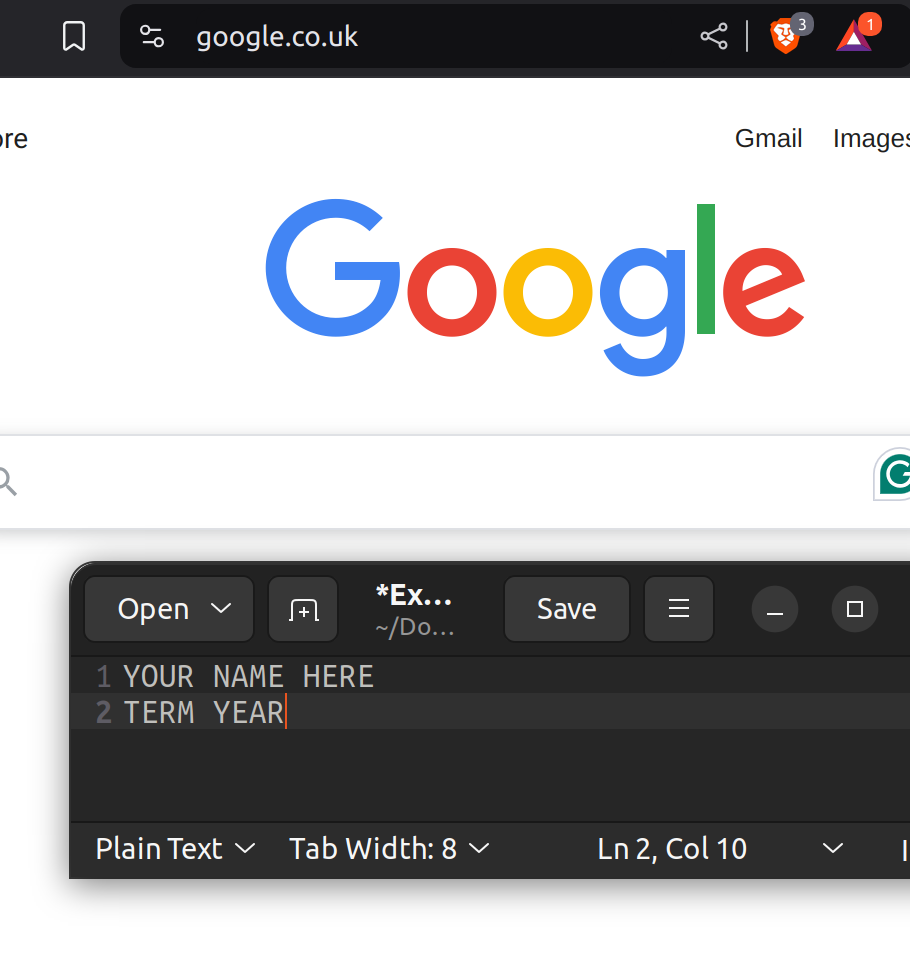
\includegraphics[scale=.2]{ExampleScreenshot.png}}
    \caption{This is an image of what each of your screenshots should look like}
    \alt{Example screenshot: a web browser showing the Google home page, with a small text editor window in front of it that says YOUR NAME HERE and TERM YEAR}
\end{figure}

\textbf{Blur or cover anything sensitive before you turn in a screenshot}, as long as your name and term note still shows. That includes:
\begin{itemize}
    \item Your Wi-Fi network name and password
    \item IP addresses and MAC addresses (the long codes like \texttt{A4:83:E7:12:9B:30})
    \item Serial numbers, and account names or email addresses
    \item Device names that include someone's name, such as ``Jordan's iPhone''
\end{itemize}

\subsection*{Part 1: Your Home's Connected Devices}
Make a list of every device in your home that connects to the internet. Think beyond computers and phones: TVs, streaming sticks, smart speakers, doorbells and cameras, printers, game consoles, smart plugs and lights, thermostats, and the router itself. If you live with other people, only include devices you're allowed to look at.
\begin{enumerate}
    \item Make a table with a row for each device, and these columns:
    \begin{itemize}
        \item The device, and who makes it
        \item Does it update automatically? (Yes, No, or Not sure)
        \item Does it have a password or PIN, and has the default one been changed?
        \item Does the maker still release updates for it? Look it up for at least 3 devices.
    \end{itemize}
    \item Find the list of connected devices on your router. You can usually find it in your internet provider's app, or the router's settings page. Take a screenshot. If you can't get to your router, such as in a dorm, say so, and take a screenshot of the Wi-Fi settings on one device instead.
    \item Pick 2 devices, and find their privacy policies. For each one, quote one thing the policy says the device collects, such as voice recordings, viewing history, or location.
    \item Which device in your home is the biggest risk? Think about what it can see or hear, whether it still gets updates, and what an attacker could do with it.
    \item Fix one thing, such as turning on automatic updates, changing a default password, or turning off a microphone or camera feature you don't use. Take a screenshot showing the change, and explain why you chose it.
\end{enumerate}

\subsection*{Part 2: Check Your Computer}
Check your own computer. Follow the steps for the kind you have. Menu names change between versions, so if you can't find something, search the device's help pages for the setting's name.

\textbf{Windows:}
\begin{itemize}
    \item \textbf{Updates:} open Settings, then Windows Update. Take a screenshot.
    \item \textbf{Secure boot:} press the Windows key, type System Information, and open it. In System Summary, find Secure Boot State. Take a screenshot. It will say On, Off, or Unsupported.
    \item \textbf{Signed apps:} open File Explorer, and go to the Program Files folder on your C: drive. Find an app's main program file, right-click it, select Properties, then the Digital Signatures tab. Take a screenshot showing who signed it.
\end{itemize}
\textbf{Mac:}
\begin{itemize}
    \item \textbf{Updates:} open System Settings, then General, then Software Update. Select the information button next to Automatic Updates, and take a screenshot.
    \item \textbf{Secure boot:} hold the Option key, open the Apple menu, and select System Information. Under Hardware, select Controller, and take a screenshot showing Secure Boot. If your Mac is older and doesn't show it, take a screenshot of About This Mac instead, and look up whether your model has secure boot.
    \item \textbf{Signed apps:} open System Settings, then Privacy \& Security, and scroll to ``Allow applications from''. Take a screenshot.
\end{itemize}
\textbf{Chromebook:}
\begin{itemize}
    \item \textbf{Updates:} open Settings, then About ChromeOS, and select Check for updates. Take a screenshot.
    \item \textbf{When updates end:} in About ChromeOS, select Additional details, and find Update schedule. Take a screenshot showing when your Chromebook gets its last update.
    \item \textbf{Secure boot and signed apps:} Chromebooks always check the system when they start, which Google calls Verified Boot, and they only install apps from the Chrome Web Store and Google Play unless you change that. You don't need a screenshot for this one. Explain it in question 8.
\end{itemize}

\subsection*{Part 3: Check Your Phone}
Check your own phone. Follow the steps for the kind you have.

\textbf{iPhone:}
\begin{itemize}
    \item \textbf{Updates:} open Settings, then General, then Software Update, then Automatic Updates. Take a screenshot.
    \item \textbf{App updates:} open Settings, then App Store, and take a screenshot of App Updates.
    \item \textbf{Secure boot and signed apps:} iPhones always use secure boot, and only install signed apps, usually from the App Store. Explain it in question 8.
\end{itemize}
\textbf{Android:}
\begin{itemize}
    \item \textbf{Updates:} open Settings, and find Software update. It's often under System. Take a screenshot showing the last security update date.
    \item \textbf{Play Protect:} open the Play Store, select your profile picture, then Play Protect. Take a screenshot.
    \item \textbf{Unknown apps:} in Settings, search for ``Install unknown apps''. Take a screenshot showing which apps are allowed to install other apps. For most people, the answer should be none, or only the Play Store.
\end{itemize}

Then answer these questions about both your computer and your phone:
\begin{enumerate}[start=6]
    \item Was anything turned off, out of date, or set in a risky way? If so, fix it if it's your device, take a screenshot, and explain what you changed. If everything was fine, say so.
    \item Does your computer or phone still get updates? Look up how long the maker supports your model, and give the source.
    \item Explain in your own words what each protection does: automatic updates, secure boot, and signed apps. For each one, give an example of an attack it helps stop, such as a fake update or malware that loads before the operating system.
\end{enumerate}

\subsection*{Part 4: Getting Rid of Old Devices}
Old devices still have data on them. Printers and copiers often store copies of what they printed or scanned, on a built-in drive.
\begin{enumerate}[start=9]
    \item Pick an old phone, computer, tablet, or printer that you or your family no longer use. If you don't have one, pick a device you use now, and plan for when you replace it.
    \item Find the maker's instructions for wiping it, such as a factory reset. Take a screenshot of the instructions. If the device is yours, backed up, and no one needs it, you can wipe it, and take a screenshot of the reset screen. Don't wipe a device someone still uses.
    \item Find a place that takes old electronics for recycling near you, or a trade-in or recycling program from the maker or a store. Give the name and link.
    \item Write a short policy, of at least 5 rules, for what a small office should do with old devices. Include computers, phones, and printers or copiers. For example: who's responsible, how devices are wiped, how wiping is checked, and where devices go after.
\end{enumerate}

\section*{Deliverables}
One file that includes:
\begin{itemize}
    \item Part 1: your device table, your router or Wi-Fi screenshot, your 2 privacy policy quotes, your answers, and your screenshot of the change you made
    \item Part 2: your computer screenshots
    \item Part 3: your phone screenshots, and your answers
    \item Part 4: your device, your screenshot of the wipe instructions, the recycling place, and your policy
\end{itemize}
Remember to blur sensitive information in every screenshot.

\section*{Resources}
References, a video, a PowerPoint and some notes are available at my website
Link: \href{https://www.aholdengouveia.name/InfoSec/PhysicalSecurity.html}{\textbf{\nolinkurl{https://www.aholdengouveia.name/InfoSec/PhysicalSecurity.html}}}

Apple: how secure boot works on a Mac with Apple silicon
Link: \href{https://support.apple.com/guide/security/secac71d5623/web}{\textbf{\nolinkurl{https://support.apple.com/guide/security/secac71d5623/web}}}

Google: check your Chromebook's update schedule
Link: \href{https://support.google.com/chromebook/answer/9367166}{\textbf{\nolinkurl{https://support.google.com/chromebook/answer/9367166}}}

FTC: how to remove your personal information before you get rid of your phone
Link: \href{https://consumer.ftc.gov/articles/how-remove-your-personal-information-you-get-rid-your-phone}{\textbf{\nolinkurl{https://consumer.ftc.gov/articles/how-remove-your-personal-information-you-get-rid-your-phone}}}

FTC: how to remove your personal information before you get rid of your computer
Link: \href{https://consumer.ftc.gov/articles/how-remove-your-personal-information-you-get-rid-your-computer}{\textbf{\nolinkurl{https://consumer.ftc.gov/articles/how-remove-your-personal-information-you-get-rid-your-computer}}}

FTC: digital copier data security, a guide for businesses
Link: \href{https://www.ftc.gov/business-guidance/resources/digital-copier-data-security-guide-businesses}{\textbf{\nolinkurl{https://www.ftc.gov/business-guidance/resources/digital-copier-data-security-guide-businesses}}}

\end{document}
